\colorlet{chaptergrey}{red!60!yellow!30!}
\chapter[Kinematics and the cosmic web]{Exploring the role of the cosmic web in galaxy evolution using kinematics}
\label{ch:halo_assembly}
\vspace{-5.25in}
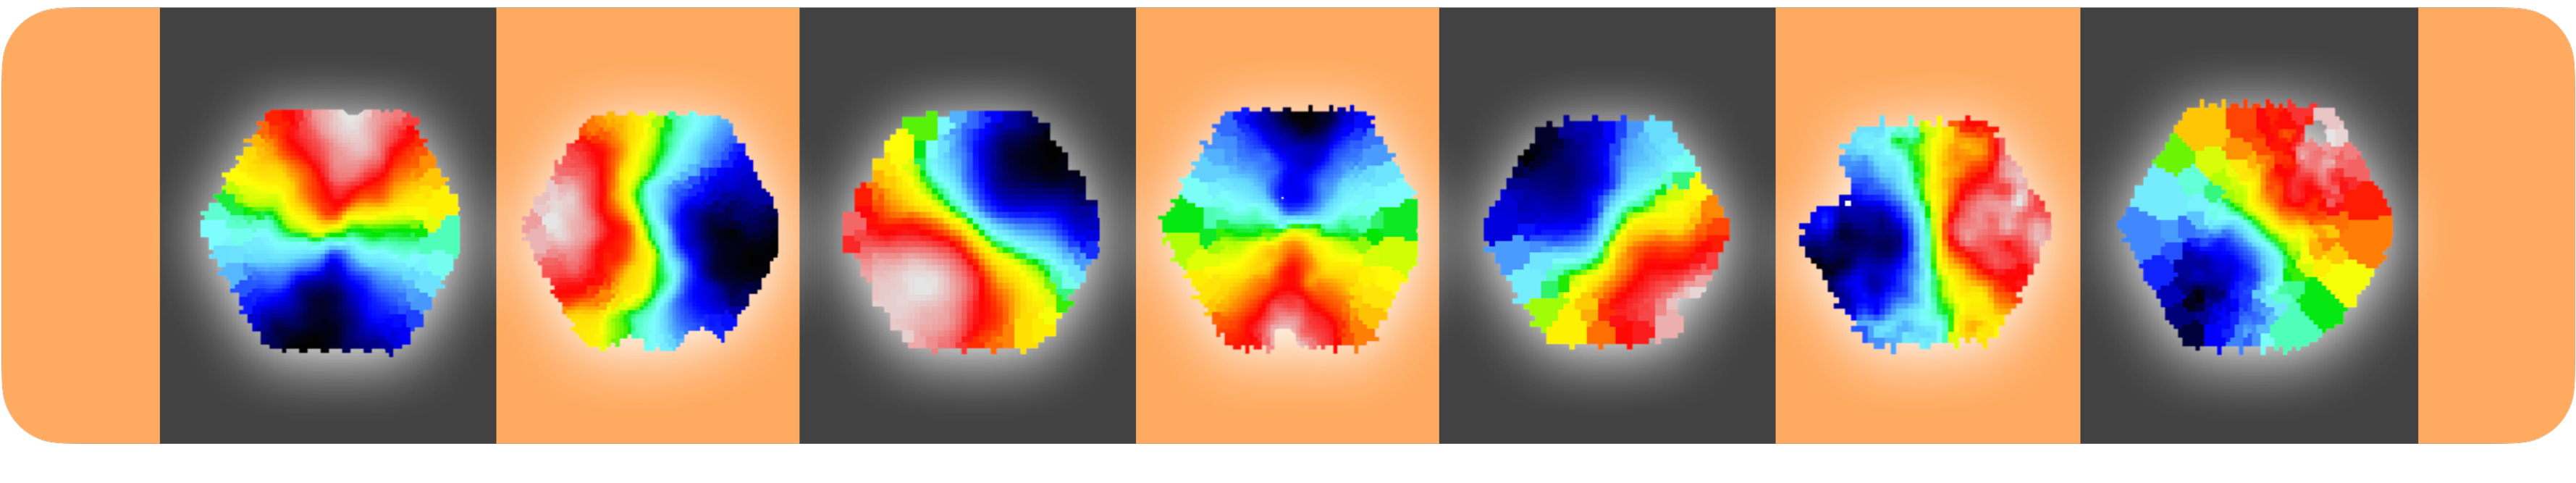
\includegraphics[height=1.33in]{thesis/latex/headers/orange_ifu.pdf}
\vspace{3in}3

\epigraph{This chapter is partially based on Kraljic, Duckworth, Tojeiro et al. (in prep.) and Duckworth, Tojeiro, Kraljic, Sgr\'o, Wild, Weijmans, Lacerna and Drory, in MNRAS, 448, Issue 1, 2019. Here, we investigate how large scale IFS surveys can be utilized to understand the relationship between galaxy kinematics and their large-scale environment.}

\section{Introduction}
In Chapters 2 and 3, we demonstrated how galaxy kinematics are closely related to morphological properties, baryonic processes such as AGN feedback, and the characteristics of its surrounding dark matter halo. The stellar (dark matter halo) mass of a galaxy encodes a lot of its evolution, demonstrating that \textit{local environment} (and over-density) can explain a large part of the diversity of properties we observe.

As introduced in \S\ref{sec:cosmic_web_intro}, galaxies on large scales are organised within the cosmic network of filamentary structure. Dark matter haloes and their constituent galaxies are subject to the large-scale anisotropic forces throughout their formation and evolution, in particular shaping their initial angular momentum content, before non-linear baryonic processes take hold. There is growing evidence that the cosmic web environment of a galaxy, also plays a significant role in galaxy evolution and is, at least partially, driving their morphology. 

Revisiting tidal torque theory \citep[TTT; e.g.][]{hoyle1951, peebles1969} in the context of large-scale anisotropic environment, \citet{codis2015} explain the relative angular momentum distribution of haloes with respect to neighbouring filaments and walls. The misalignment between the inertia tensors of the proto-haloes and the directionality of the tidal tensor due to the neighbouring wall or filament leads to a spin alignment for low mass haloes. As these haloes grow in mass hierarchically, merging with other haloes and they lose this preferential alignment with large scale structure. Due to the flow of matter along walls and filaments, mergers often happen in this plane, possibly leading to a \textit{flip} in direction, so that higher mass dark matter haloes are preferentially perpendicular to the orientation of the tidal field \citep[e.g.][]{Codis2012, dubois2014, GaneshaiahVeena2018}. This understanding is motivated by cosmological N-body simulations and learning how this propagates to observations is complex. In simulations, the constituent galaxies appear to retain a memory of the spin orientation (with respect to large scale structure) as dictated by their host dark matter halo \citep[e.g.][]{codis2018, Kraljic2019flip}. The mass dependence of the spin alignment \textit{flip} is, however, debated and likely dependent on different choices for baryonic processes and the scale of the neighbouring filamentary structure. The orientation of galaxies with respect to large-scale structure is, however, only one aspect in determining the relationship between galaxy evolution and the cosmic web. In this theoretical framework, it could be expected that not only the spin alignment, but also, the spin \textit{magnitude} of a given galaxy would be modulated as function of its position within the cosmic web.

A powerful approach in a holistic understanding of galaxy evolution, and hence, potentially enabling us to trace the impact of the cosmic web, is spatially resolved spectroscopy. As introduced in \S\ref{sec:ifs_surveys_intro} IFS surveys for thousands of galaxies, across a wide variety of morphologies, environments, and masses in the local Universe are now a reality. Current generation IFS surveys such as MaNGA and SAMI have opened the door for a detailed understanding between kinematics, morphology, and, stellar mass ($\mathrm{M_{stel}}$). 

Using data from the SAMI IFS survey, \citet{cortese2016} demonstrated that the angular momentum of both stars and gas correlates strongly positive with stellar mass. For galaxies with $\mathrm{M_{stel} > 10^{9.5} M_{\odot}}$, the scatter in the $\mathrm{M_{stel}}$ - angular momentum relationship can be constrained by optical morphology (i.e. sersic index). This scatter, however, can be even more strongly correlated with $\mathrm{\lambda_R}$ (as defined in equation \ref{eq:lambda_R}; here only calculated within 1\re). These tight relationships indicate that early-type fast rotators and late-type galaxies are not two separate classes of objects, but represent a `continuum' connecting pure-disks to bulge-dominated systems. In MaNGA, \citet{graham2018} investigate the relationship between angular momentum and optical morphology for $\sim$2300 galaxies. They demonstrate that both stellar mass and morphology correlate strongly with the stellar angular momentum of galaxies. Furthermore, they use $\mathrm{\lambda_R}$ and ellipticity to separate early-type galaxies into fast and slow rotators, finding a clear bi-modality in their distribution, and hence, potentially highlighting their different assembly histories. 

The relationship between stellar angular momentum and environment in observations is, however, less clear. In MaNGA, \citet{greene2018} make use of the \citet{yang2007} group catalogue (introduced in \S\ref{sec:group_def}) to define halo mass and separate galaxies into central and satellites. They find minimal evidence that $\mathrm{\lambda_R}$ / $\epsilon^{0.5}$ (i.e. stellar angular momentum normalised by shape) depends on the mass of the group, once the role of $\mathrm{M_{stel}}$ has been accounted for. They also find minimal difference between centrals and satellites, in terms of slow rotator fraction. \citet{wang2020} demonstrate that the environmental dependence of stellar angular momentum is significantly weaker than the stellar mass dependence. While there is no particular trend with halo mass for low mass galaxies, high mass ($\mathrm{M_{stel} > 10^{10.9} M_{\odot}}$) central galaxies (or those in dense/rich groups) have lower $\mathrm{\lambda_R}$. Extending this idea, \citet{graham2019} use 3900 galaxies in MaNGA to demonstrate that the fraction of galaxies defined as slow rotator \textit{does} increase with overdensity, however, there is a more marked effect when comparing to the relative density (i.e. correlating with the relative peak densities, rather than absolute which averages signal out). Even further, using distance to cluster/group centre shows the strongest trends with slow rotator fraction, suggesting a direct link with SR creation (from dry merger events and are selected to be $\mathrm{M_{stel} > 2\times10^{11} M_{\odot}}$) and cluster cores. This holds true at fixed stellar mass ($\mathrm{M_{stel} > 2\times10^{11} M_{\odot}}$). How the spin magnitude of galaxies is modulated by \textit{large-scale} environment, however, is a topic in its infancy at the time of writing (observationally). In this chapter, we use the MaNGA survey to explore two questions:

\begin{itemize}
    \item How does the magnitude of stellar angular momentum in galaxies depend individually on morphology, halo mass, and, large scale structure?
    \item Does the spin orientation of galaxy disks in the local Universe align with the local geometry of neighbouring filaments?
\end{itemize}

In \S\ref{sec:spin_magnitude} we investigate how the stellar angular momentum content of galaxies in MaNGA is dependent on local and large-scale environment. We make use of the largest IFS galaxy sample to date (MPL-9; exactly 8000 unique galaxies before cross-matching), to understand how galaxy spin is modulated with respect to different morphological features of the cosmic web once stellar mass, and, morphology have been accounted for. We also consider how group membership and halo mass can drive individual changes in the angular momentum content. In \S\ref{sec:spin_alignment} we present the first study making use of galaxy kinematics to estimate the 3D alignment between the spin direction of galaxy disks and their neighbouring filamentary structure. We investigate the dependence of spin alignment on stellar mass and galaxy morphology, to better understand the connection between galaxy evolution and the cosmic web. We summarise and conclude in \S\ref{sec:cw_spin_conclusion}.

\subsection{Data and Methods}
\subsubsection{Galaxy sample}
In \S\ref{sec:spin_magnitude}, we base our analysis on 8000 unique galaxies corresponding to the 9th MaNGA product launch. In contrast, we make use of 4633 unique galaxy observations (MPL-6) for \S\ref{sec:spin_alignment}, reflecting the state of the survey as of mid-2018 (data released publicly December 2018). This is also our defined sample in the following chapter. 

Specific to \S\ref{sec:spin_alignment}, for each galaxy we compute kinematic position angles for both the stellar and ionized gas velocity fields. We calculate position angles as described in \S\ref{sec:kin_mis}. In this section, concerning spin alignment, we only make use of position angles derived from stellar kinematics.
%, however, in \S\ref{sec:halo_assembly} we make use of the full kinematic misalignment measures. 
Throughout this chapter, we select our sample based on the visual morphological classifications of GalaxyZoo2 \citep[GZ2][]{willett2013} as introduced in \S\ref{sec:morph_def_obs}. For the purpose of \S\ref{sec:spin_magnitude}, we select the same vote thresholds as chapter 2 (i.e. $P = 0.7$ for a given morphological feature). In \S\ref{sec:spin_alignment}, to compute the spin direction of each galaxy in our sample, we assume a thin disk approximation (see \S\ref{sec:thin_disk}) and therefore we require each galaxy to have a well defined disk component. For this purpose, we select a \textit{pure} spiral galaxy sample by taking all objects that have a debiased vote fraction of $\geq 0.9$ for answers positive to the galaxy having a disk. \red{add in lenticular definition}.

\subsubsection{DisPerSE}
For all work in this chapter (and Chapter 5), we characterise the topological features of the cosmic web using the Discrete Persistent Structure Extractor Code \citep{sousbie2011a, sousbie2011b} as introduced in \S\ref{sec:cosmic_web_intro}. Here DisPerSE is applied to a modified version of the SDSS DR10 spectroscopic sample as described in \citet{tempel2014}. In observations, there is an additional difficulty since we are not working with exact three dimensional positions in real space, but rather, in redshift space. To recover the intrinsic galaxy position, an estimation for the peculiar velocity must be made for each galaxy. On large-scales this corresponds to the Kaiser effect \citep{kaiser1987}, which acts to increase the contrast of the skeleton due the coherent motion of galaxies with the growth of structure \citep[e.g.][]{shi2016}. On small-scales, however, the Fingers of God effect \citep[FOG;][]{jackson1972,tulley1978} derives from random motions of galaxies within virialized haloes. The latter can elongate structure in redshift space leading to erroneous identification of filaments. We correct for the FOG effect using the technique outlined in \citet{kraljic2018}. As introduced in \S\ref{sec:cosmic_web_intro}, the \textit{robustness} of the cosmic web's morphological features identified are quantified using the so called persistence ratio, a measure of the significance of the topological connection between individual pairs of critical points. Here we use choose robust filaments identified with a significance of 5$\sigma$. In Figure \ref{fig:disperse_sdss} we show an example of the recovered density field from the set of galaxy positions in SDSS and the corresponding ridge extraction (i.e. filament detection). \red{length of typical segments with respect to typical distance to galaxy?}

\begin{figure*}
    \centering
	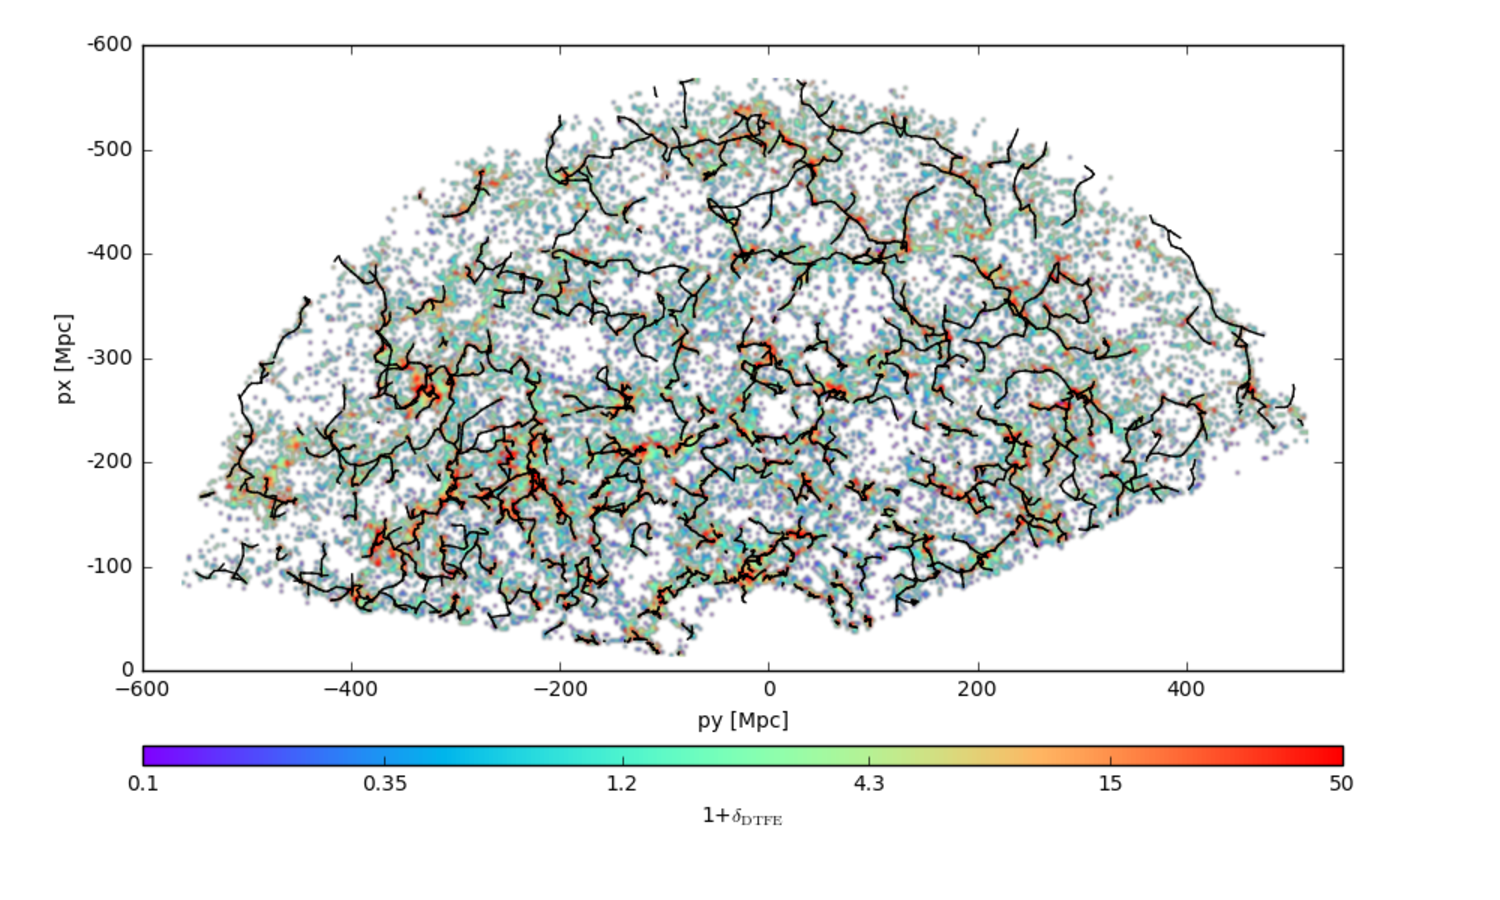
\includegraphics[width=\linewidth]{thesis/latex/halo_assembly_manga/SDSS_CW_DisPerSE.pdf}
    \caption[Illustration of the filamentary network for a slice of the SDSS field.]{Illustration of the filamentary network (black lines) for a slice of the SDSS field ($0.02 \leq z \leq 0.15$; $ 27 \leq$ dec $\leq 33$) extracted using the DisPerSE code. Only filamentary structures which are seen to persist above the 5$\sigma$ threshold are shown, along with the density contrast of the galaxy population. The density contrast is estimated using the small-scale DTFE estimator (see text). Adapted from \citet{duckworth2019_halo}, with credit to K. Kraljic.}
    \label{fig:disperse_sdss}
\end{figure*}

The local geometry of each filament is characterised by a series of smaller \textit{segments}, which are the default output of the DisPerSE code. For each galaxy, the nearest segment is found and its direction is used to compare to the given galaxy's spin direction. 

\subsubsection{Cosmic web distances} \label{sec:cosmic_web_distances}
Having constructed a skeleton of the cosmic web, a galaxy's environment can be described by finding its vicinity to various features of the skeleton. The cosmic web comprises of low density `void' regions which are enclosed by `walls' of structure which become filaments at points of intersection. The gravitational potential of the filaments dictate the flow of the matter, which at the point of intersection, feed high density regions interpreted as `nodes'. Along the filament, saddle points remain as minima between the flows towards nodes. 

The distance to the nearest filamentary point, $D_{skel}$, is first found for each galaxy. To then consider the influence of the nearest node, the distance from this impact point along the filament to the node is also computed, $D_{node}$. Finally the distance to the nearest wall, $D_{wall}$, can then be found. In order to investigate expected trends of galaxies with vicinity to any cosmic web feature we must remove effects resulting due to the proximity of others. For $D_{skel}$ we remove all galaxies that lie within $D_{node} < 0.5$ Mpc. 
% and for $D_{wall}$, all galaxies within $D_{node} < 0.5$ Mpc and $D_{skel} < 2.5$ Mpc are discounted. 
This represents a compromise between eliminating the effect of other cosmic web features and having enough galaxies left to construct a statistically significant sample. Tightening the condition with respect to nodes so that we require $D_{node} > 1$ Mpc does not change any of the results presented in this work. \red{find out maximum distance at which a galaxy is considered to be connected with a filament in Kat's sample.}

Construction of the cosmic web from any observation is influenced by the completeness and the sampling of the galaxy sample. The modified SDSS DR10 spectroscopic sample is complete to $m_r$ = 17.77. A sample containing only brighter galaxies will naturally only identify stronger/larger filamentary features and hence smaller substructures will be missed. In addition, the lower the sampling of galaxies, the lesser the accuracy of the actual position of cosmic web features. To correct for this, the distances are normalised by the mean inter-galaxy separation, $\left\langle D_z \right\rangle$ at a given redshift, as such $\left\langle D_z \right\rangle = n(z)^{-1/3}$ where $n(z)$ is the number density. \red{rewrite this paragraph}

\section{Spin magnitude} \label{sec:spin_magnitude}

\subsection{Morphology}

\begin{figure}
    \centering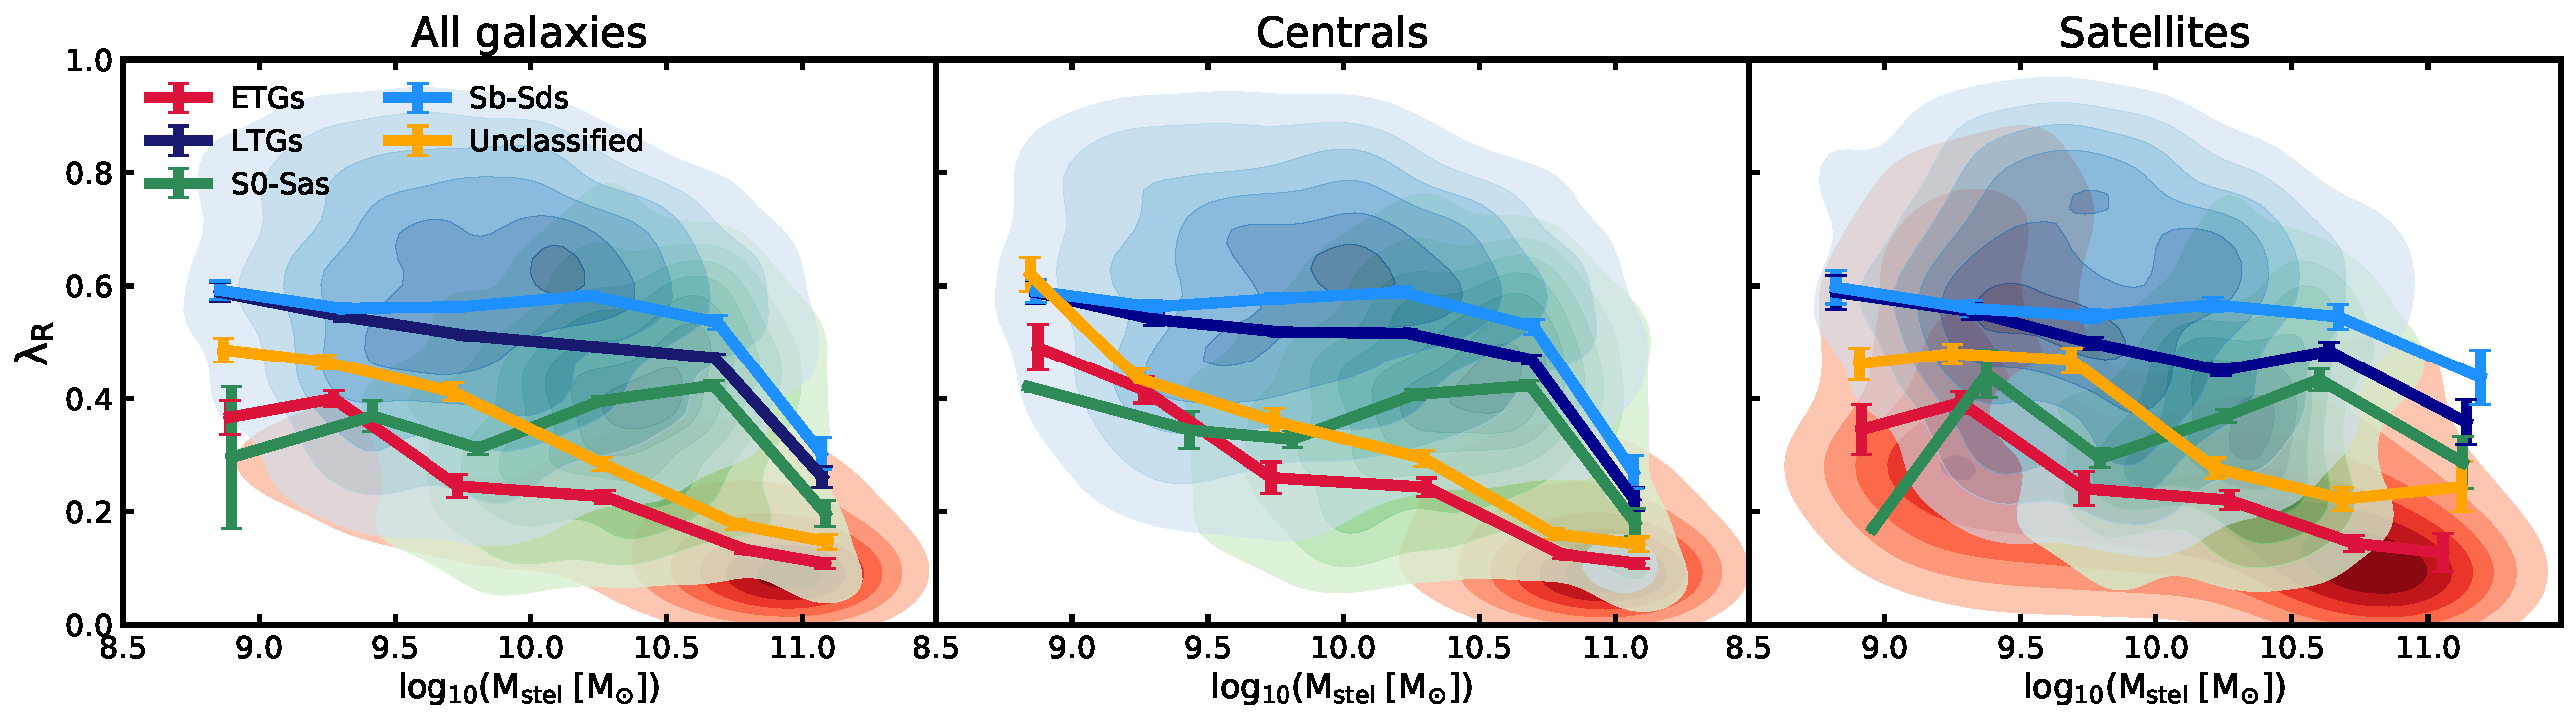
\includegraphics[width=\linewidth]{thesis/latex/cw_spin/morphology_lambdaR_mstel_kde_wo_unclassified.pdf}
    \caption{Distribution of angular momentum (\lambdaR) as a function of stellar mass (\mstel) for all ETGs (red), LTGs (dark blue), S0-Sas (green), Sb-Sds (light blue) and unclassified (orange) in MaNGA. The panels (left to right) shows the distributions for all galaxies, centrals only and satellites only respectively. In each panel, the overall distribution for ETGs, S0-Sas and Sb-Sds is shown by the contours using a KDE (see text), with average \lambdaR values shown in bins of \mstel. For all galaxies there is distinct trend with morphology and \lambdaR  with later types being higher angular momentum than earlier types at all masses. There is also a correlation between \lambdaR  and \mstel  for each morphological type, with galaxies in higher mass haloes typically having lower angular momentum.}
\label{fig:morph_lambdaR_mstel}
\end{figure}

\begin{figure}
    \centering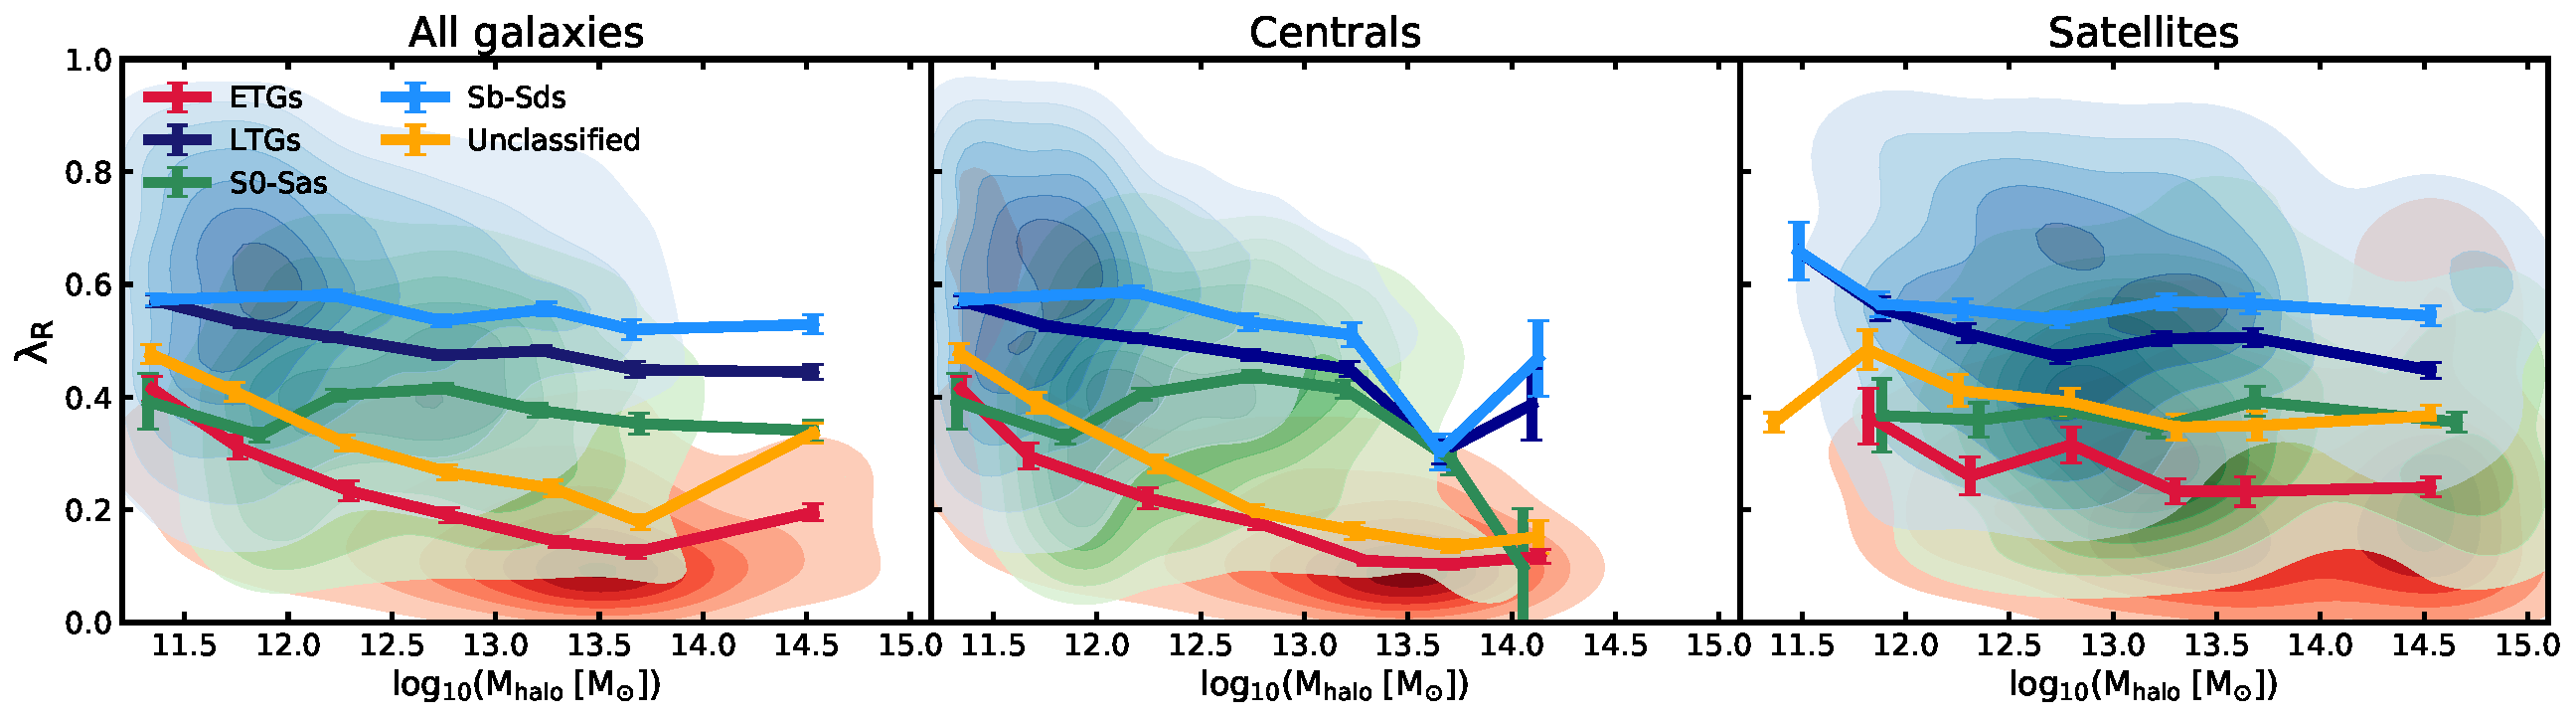
\includegraphics[width=\linewidth]{thesis/latex/cw_spin/morphology_lambdaR_mhalo_kde_wo_unclassified.pdf}
    \caption{Distribution of angular momentum (\lambdaR) as a function of halo mass (\mhalo) for all ETGs (red), LTGs (dark blue), S0-Sas (green), Sb-Sds (light blue) and unclassified (orange) in MaNGA. The panels (left to right) shows the distributions for all galaxies, centrals only and satellites only respectively. In each panel, the overall distribution for ETGs, S0-Sas and Sb-Sds is shown by the contours using a KDE (see text), with average \lambdaR values shown in bins of \mhalo. For all galaxies there is distinct trend with morphology and \lambdaR  with later types being higher angular momentum than earlier types at all masses. There is also a correlation between \lambdaR  and \mhalo for each morphological type, with galaxies in higher mass haloes typically having lower angular momentum.}
\label{fig:morph_lambdaR_mhalo}
\end{figure} 

\subsection{Group membership}

\begin{figure}
    \centering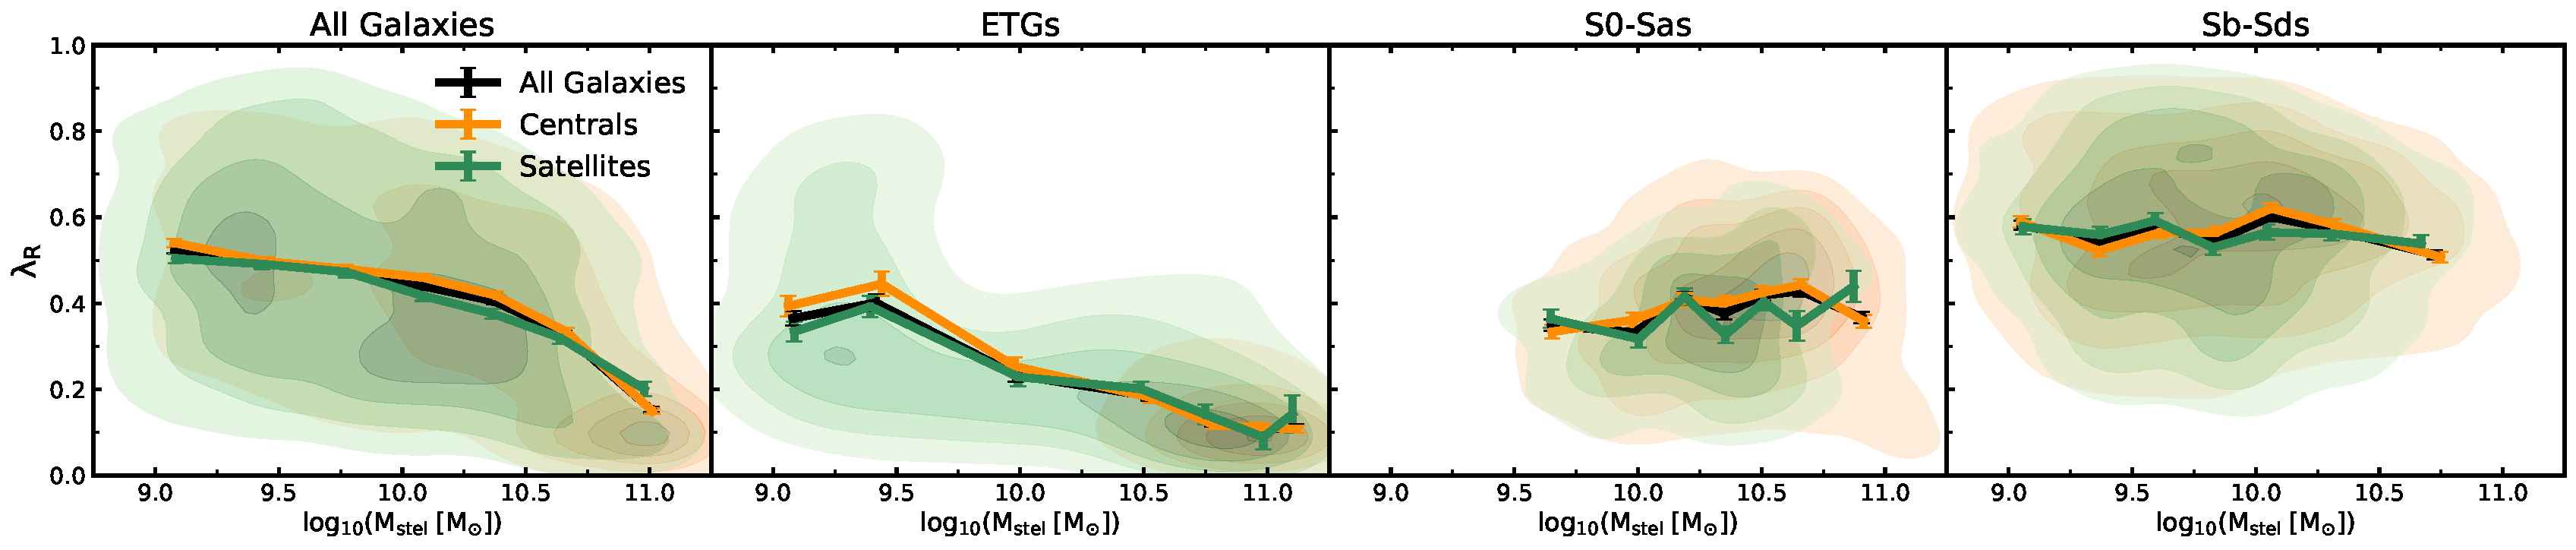
\includegraphics[width=\linewidth]{thesis/latex/cw_spin/group_lambdaR_mstel.pdf}
    \caption{}
\label{fig:}
\end{figure} 

\begin{figure}
    \centering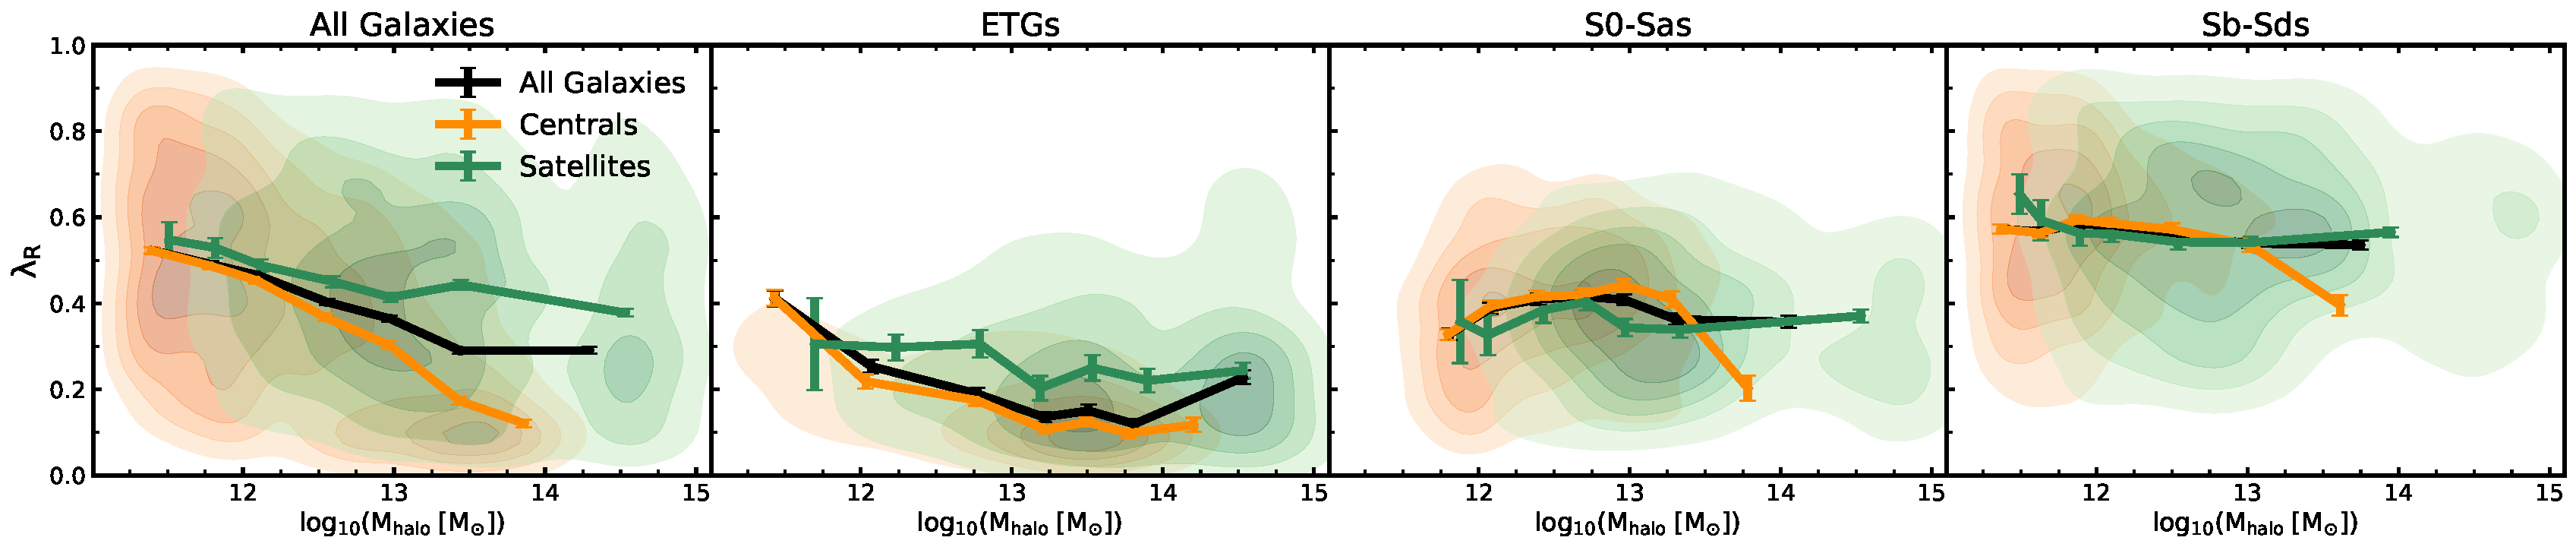
\includegraphics[width=\linewidth]{thesis/latex/cw_spin/group_lambdaR_mhalo.pdf}
    \caption{}
\label{fig:}
\end{figure} 

\subsection{Cosmic web}

\begin{figure}
    \centering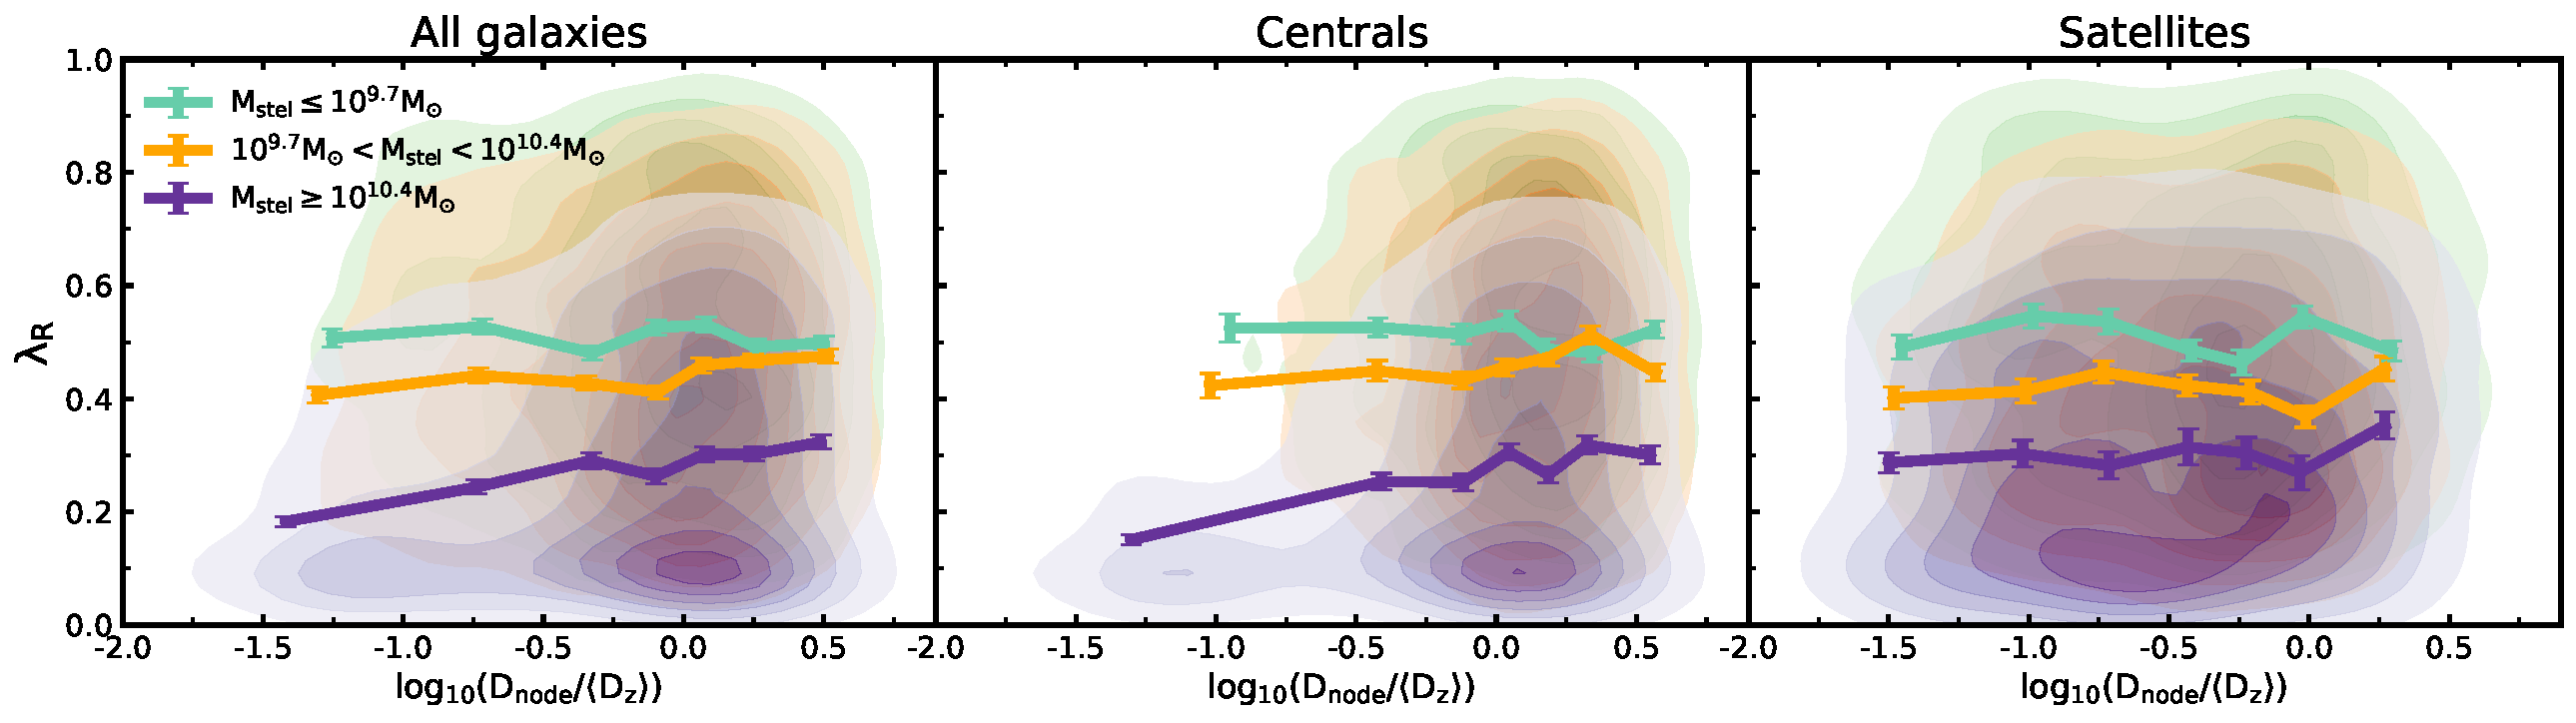
\includegraphics[width=\linewidth]{thesis/latex/cw_spin/lambdaR_dnode_mass_split_3sigma.pdf}
    \caption{}
\label{fig:}
\end{figure} 

\begin{figure}
    \centering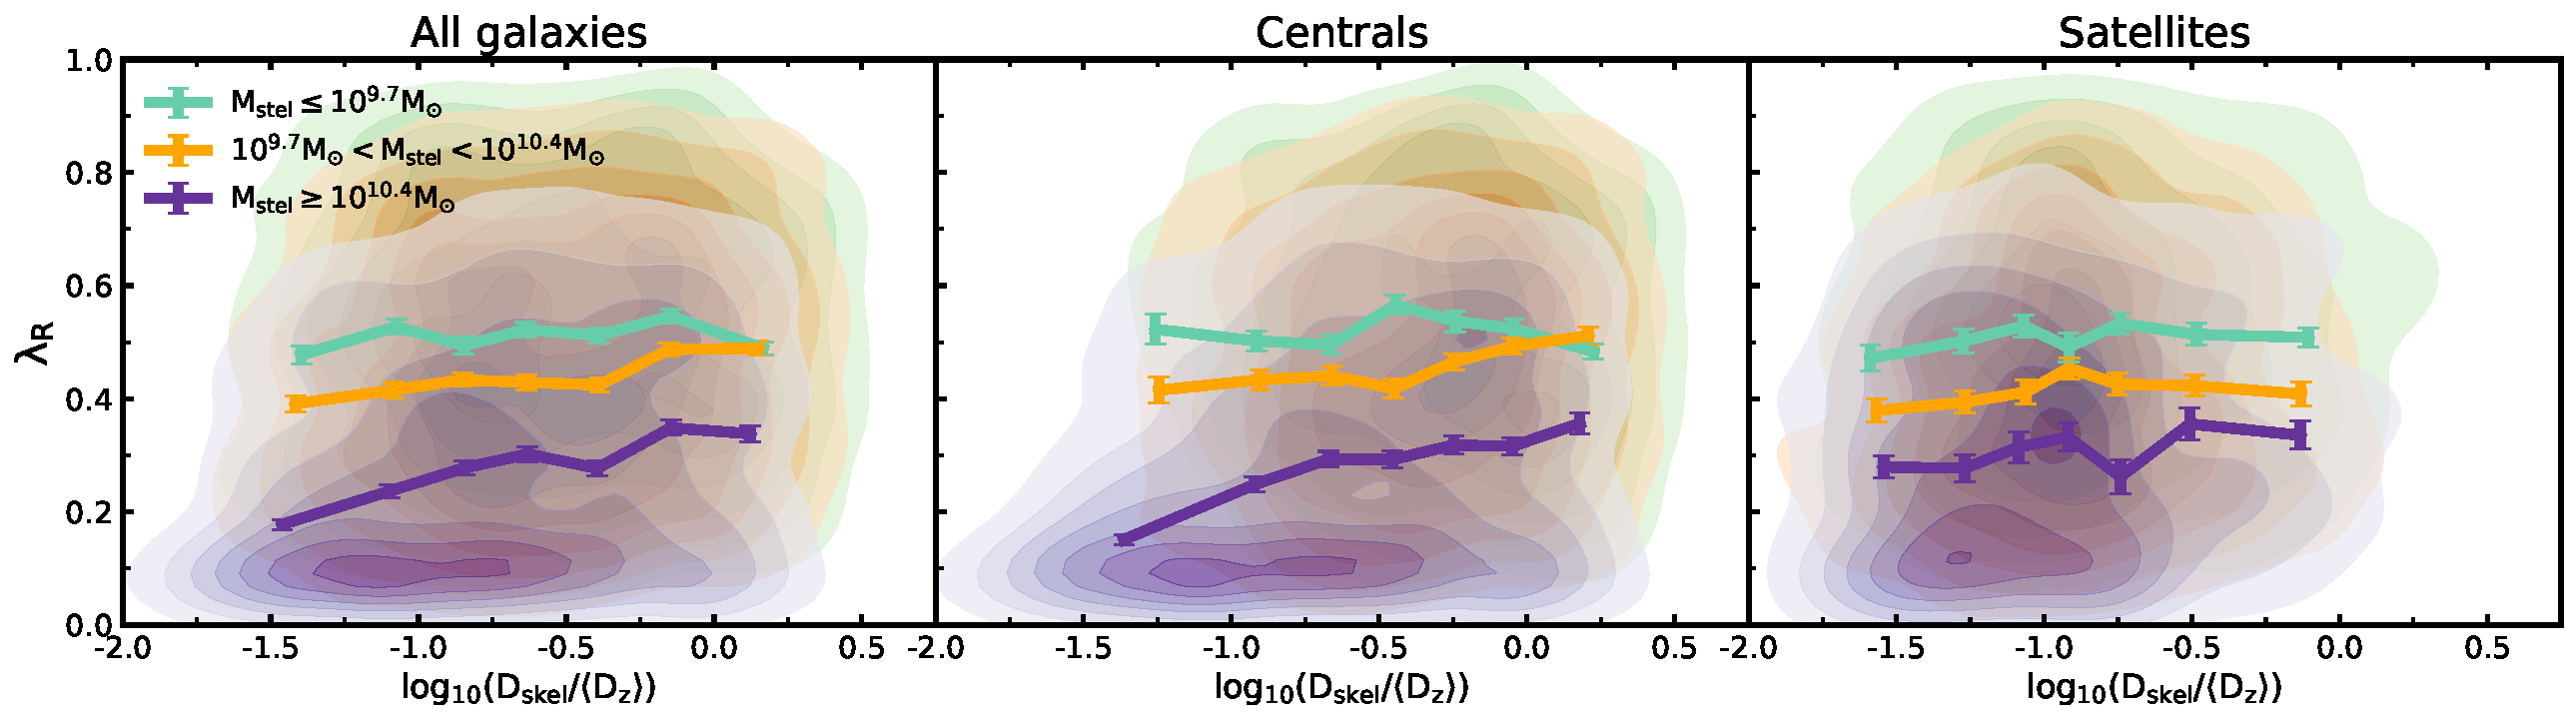
\includegraphics[width=\linewidth]{thesis/latex/cw_spin/lambdaR_dskel_mass_split_3sigma.pdf}
    \caption{}
\label{fig:}
\end{figure} 

\begin{figure}
    \centering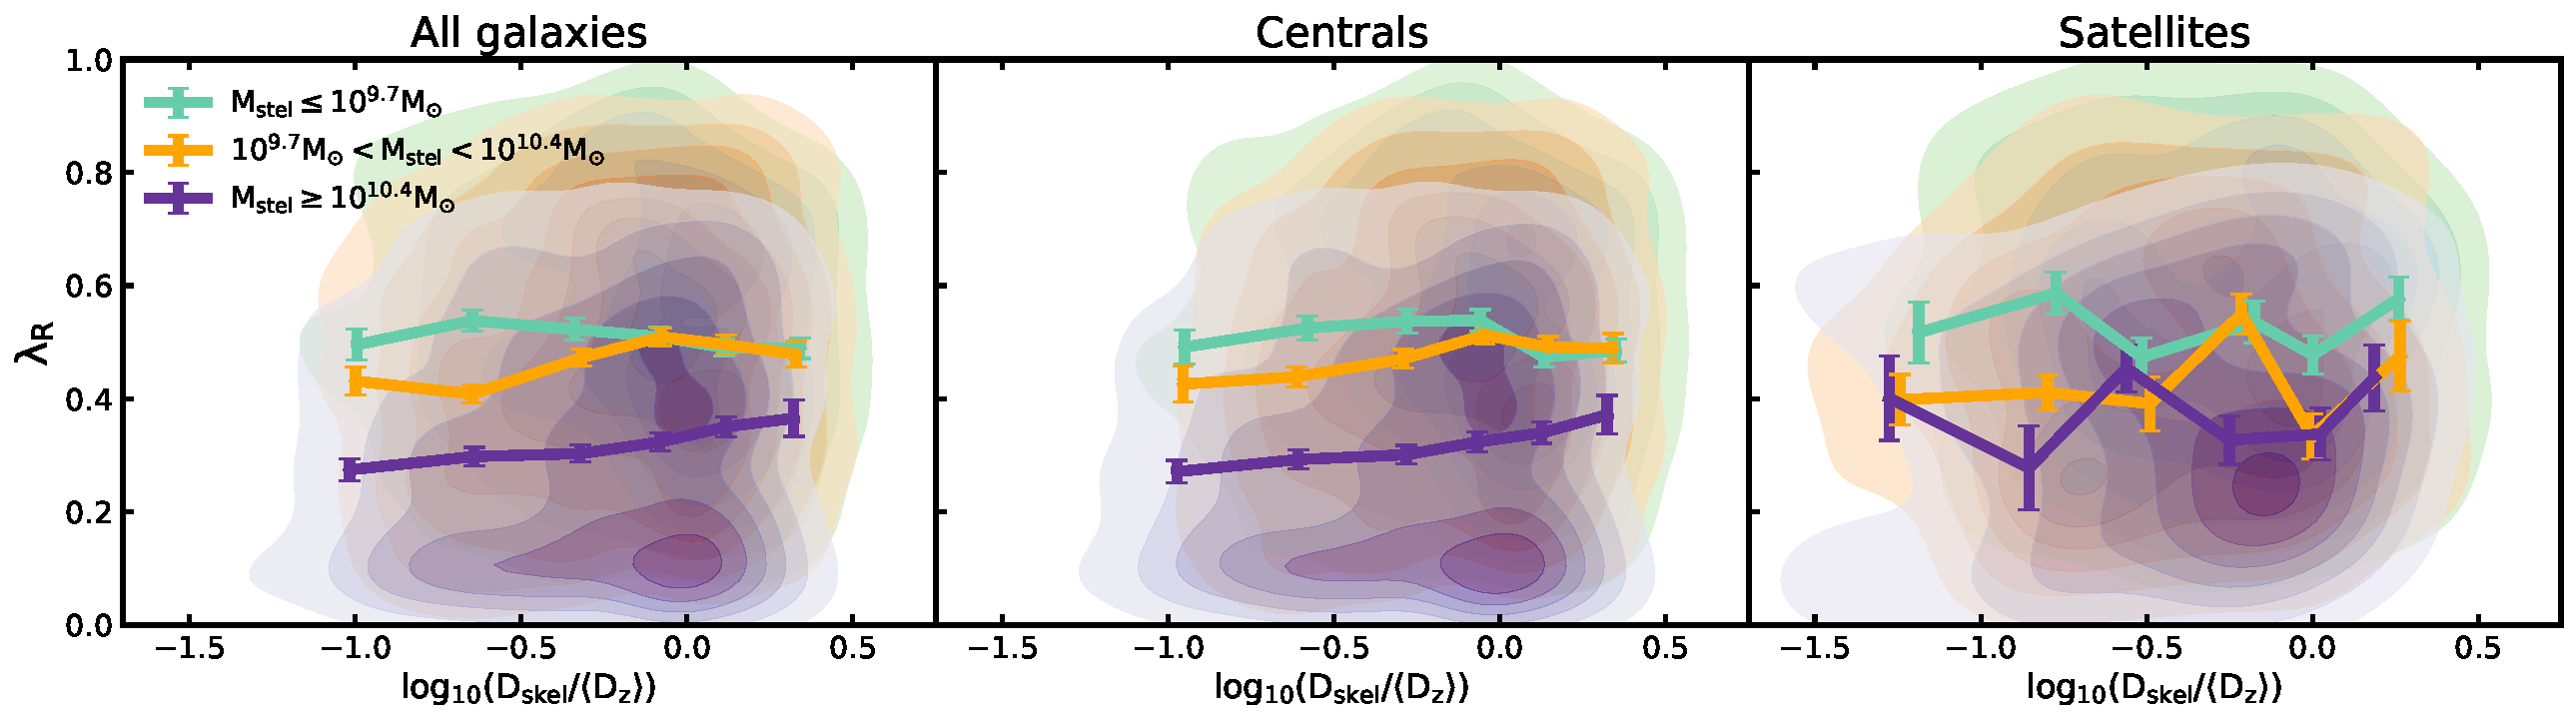
\includegraphics[width=\linewidth]{thesis/latex/cw_spin/lambdaR_dskel_no_node_mass_split_3sigma.pdf}
    \caption{}
\label{fig:}
\end{figure} 

\section{Spin alignment of spiral and S0 galaxies in MaNGA} \label{sec:spin_alignment}
\red{add figure of spin orientation with disperse overlay?}
Historically, exploring the relationship between the spin direction of galaxies and large scale structure has been difficult. Without spatially resolved spectra of galaxies, we are reliant on projected shapes, which introduce degeneracies with respect to the actual spin vector direction \citep[e.g. see Fig 2. in][for example of degeneracies that can occur]{motloch2020}. Due to this, and the different approaches to re-constructing the cosmic web, studies are often conflicting in findings \citep[e.g. spiral galaxies having parallel vs perpendicular orientations with respect to the cosmic web][]{tempel2013a, tempel2013, lee2007, jones2010, zhang2015}. These differences due to the reconstruction of the cosmic web can likely be explained due a difference in chosen scales. In hydrodynamical simulations, the transition mass from preferential parallel alignment to perpendicular alignment is very much dependent on the scale of the filamentary structure, such as width \citep{ganeshaiahveena2019, Kraljic2019flip}. Averaging over an ensemble of filamentary scales will likely wash out this transition, and hence preferential alignment in either direction. 

The other half of the problem can be solved, however, by having kinematic information for a large population of galaxies. Kinematic (rotational) position angles help break the degeneracy of shape orientation, and provide more robust measures of directionality. We are now in the era of multiple IFS surveys that may observe enough galaxies to find a significant detection of spin alignment. In this section we explore the concept of spin alignment in MaNGA for spirals and S0 galaxies.

\subsubsection{Angular momentum directions} \label{sec:thin_disk}
In order to estimate the spin direction of our galaxy sample, we assume a thin-disk approximation according to \citet{LeeErdogdu2007}. Here we summarise the key steps in calculating the three dimensional vector. Working in spherical coordinates in the reference frame of the galaxy, the spin direction can be described as
\begin{equation}
\begin{split}
\mathrm{\hat{L}_r & = \cos i,} \\
\mathrm{\hat{L}_{\theta} & = (1 - \cos^2 i)^{1/2} \sin PA,} \\
\mathrm{\hat{L}_{\phi} & = (1 - \cos^2 i)^{1/2} \cos PA,}
\end{split}
\end{equation}
where $\mathrm{PA}$ is the position angle from the stellar kinematics and $i$ is the inclination of the galaxy, defined as such
\begin{equation}
\mathrm{\cos^2 i = \frac{(b/a)^2 - p^2}{1 - p^2},}
\end{equation}
where $b/a$ is the sky projected axis ratio and $p$ is the intrinsic flatness of the galaxy \citep[varies as a function of morphology as described in][]{haynes1984}. $p$ accounts for the fact that the disk of galaxies has a finite thickness, and the presence of a bulge impacts the estimation of $b/a$. In this work we adopt an intermediate value (0.158), however choosing more extreme proposed values (0.1 - 0.23) does not change our findings. The value of $i$ is set to $\pi/2$ if $b/a < p$.

The spin direction can then be transformed into equatorial Cartesian coordinates as follows:
\begin{equation}
\begin{split}
    \hat{L}_x & = \hat{L}_r \sin \alpha \cos \beta + \hat{L}_{\theta} \cos \alpha \cos \beta - \hat{L}_{\phi} \sin \beta \\
    \hat{L}_y & = \hat{L}_r \sin \alpha \sin \beta + \hat{L}_{\theta} \cos \alpha \sin \beta + \hat{L}_{\phi} \cos \beta \\
    \hat{L}_z & = \hat{L}_r \cos \alpha - \hat{L}_{\theta} \sin \alpha
\end{split}    
\end{equation}
where $\alpha = \pi/2 - {\rm dec}$ and $\beta = {\rm RA}$.

\subsubsection{LTGs}
\begin{figure}
    \centering
    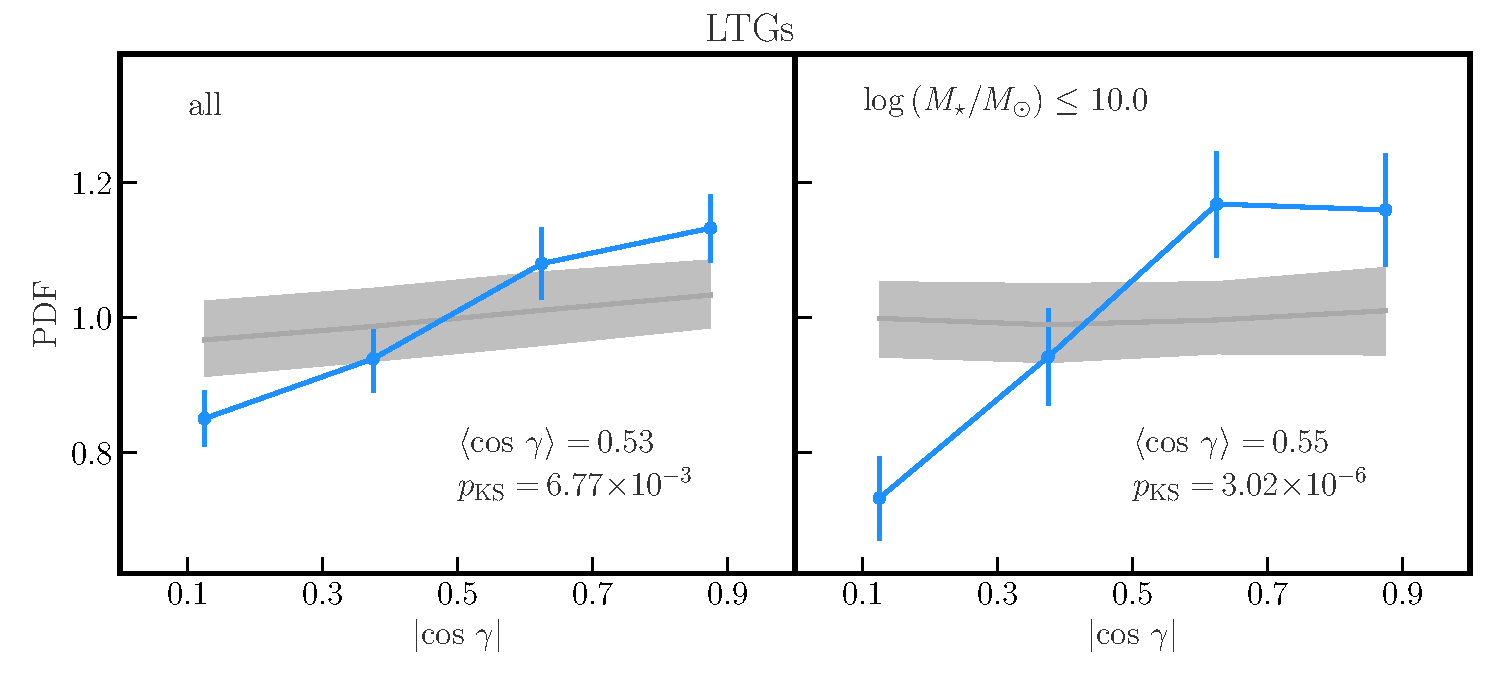
\includegraphics[width=\linewidth]{thesis/latex/cw_spin/spin_fil_LTGs_2in1.pdf}
    \caption{Alignment between neighbouring filament and spin direction of late type galaxies calculated from the thin disk approximation. Each panel shows the probability density distribution (blue) of the cosine angle between the direction of the filament segment and the spin direction. Errors are calculated through bootstrapping and the grey line (with associated errors) corresponds to the expected distribution for a completely random alignment. In addition, each panel shows the mean $\cos \gamma$ for the population and the $p$-value for a Kolmogorov--Smirnov test. The left panel shows for all LTGs in our sample, whereas the right panel shows the distribution only for those with a stellar mass $< 10^{10} M_{\odot}$. We find that for all masses LTGs are preferentially \textit{parallel} orientated with respect to the neighbouring filament, with low mass showing a more significant alignment signal.}
    \label{fig:ltgs_spin_alignment} 
\end{figure}

In Figure \ref{fig:ltgs_spin_alignment}, we show the probability density function of alignment between the spin directions of LTGs and their neighbouring filament segment. We define $\gamma$ as the angle between the spin direction and segment directions. The PDF is presented as $|\cos \gamma|$ so that 0 corresponds to exact perpendicular alignment and 1 exact parallel alignment. Each panel shows the distribution for LTGs (blue) with associated bootstrap errors, along with the expectation of the distribution if the spin vectors have completely random orientations (grey line with errors). In addition, each panel shows the mean $\cos \gamma$ for the population and the $p$-value for a Kolmogorov--Smirnov (KS) test between the LTGs and the random orientations. A KS test evaluates if two sub-populations are drawn from the same distribution with the null hypothesis that they are consistent. A low $p$-value therefore signifies that the populations are independent to the significance level stated. 

In the left panel, we show the orientations for all LTGs selected in our sample. We find that the spin of LTGs are preferentially orientated \textit{parallel} to the direction of the neighbouring filament segment, to the significance level of $p_{KS} = 6.77 x 10^{-3}$. In the right panel, we show the PDF for only LTGs that are below a stellar mass of $\mathrm{M_{stel} < 10^{10} M_{\odot}}$. Again we find a preferential parallel alignment, however, now to an increased significance level of $p_{KS} = 3.02 x 10^{-6}$. In addition $\langle \cos \gamma \rangle$ increases from 0.53 (all LTGs) to 0.55 (low mass LTGs), indicative that this signal is strongest for the low mass LTGs. This parallel alignment is in-keeping with theoretical expectation that the formation of low mass disks tend to align with the large-scale tidal field in which they evolve. 

\subsubsection{S0s}
\begin{figure}
    \centering
    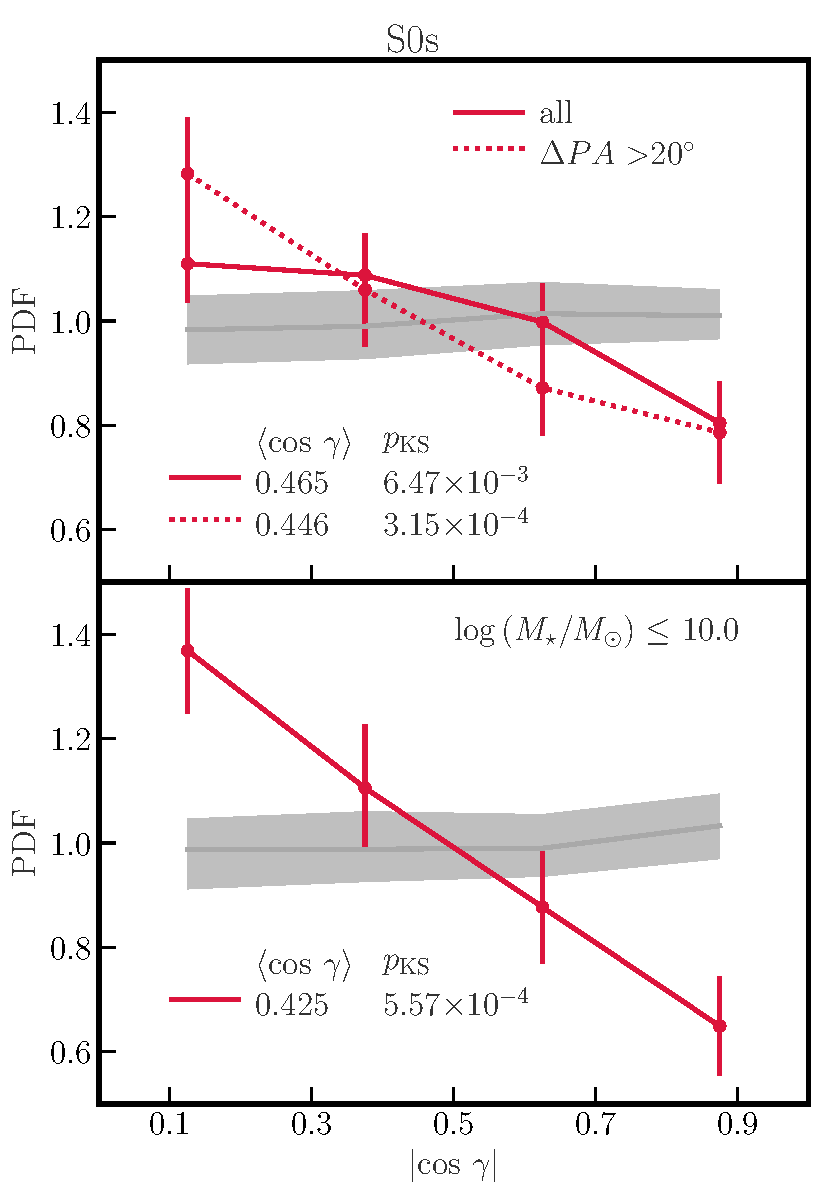
\includegraphics[width=\linewidth]{thesis/latex/cw_spin/spin_fil_S0s_2in1.pdf}
    \caption{Alignment between neighbouring filament and spin direction of lenticular galaxies calculated from the thin disk approximation. Each panel shows the probability density distribution (red) of the cosine angle between the direction of the filament segment and the spin direction. Errors are calculated through bootstrapping and the grey line (with associated errors) corresponds to the expected distribution for a completely random alignment. In addition, each panel shows the mean $\cos \gamma$ for the population and the $p$-value for a Kolmogorov--Smirnov test. The left panel shows for all S0s in our sample, whereas the right panel shows the distribution only for those with a stellar mass $< 10^{10} M_{stel}$. We find that for all masses lenticulars are preferentially \textit{perpendicular} orientated with respect to the neighbouring filament, with low mass showing a more significant alignment signal.}
    \label{fig:s0_spin_alignment}
\end{figure}

In Figure \ref{fig:s0_spin_alignment}, we now show the PDF of alignment between the disks of lenticular galaxies and their neighbouring filament segment. As before, we show the PDF as a $\cos \gamma$ distribution with the left panel showing the results for all S0s in our sample and the right for low mass ($\mathrm{M_{stel} < 10^{10} M_{\odot}}$) S0s only. Here, we find that the spin direction of S0s are preferentially \textit{perpendicular} with respect to their neighbouring filament segment. Considering the null hypothesis that the spin directions have random orientation, we find that the total S0 population is different from random to a significance of $p_{KS} = 8.56 x 10^{-3}$ which increases to  $p_{KS} = 8.37 x 10^{-4}$ when only considering the low mass S0s. This preferential perpendicular alignment could be indicative of the evolutionary history of lenticular galaxies embedded in large filamentary structure. The expectation from N-body simulations is that the orientation of dark matter haloes flip in direction due to mergers in the plane of the filament. This could be indicative that the S0s near filamentary structure have undergone mergers in their recent history, leading to a perpendicular orientation. 

\subsection{Discussion and Summary} \label{sec:cw_spin_conclusion}
Of most relevance to our findings are the studies of spin alignment which also make use of large scale IFS surveys. In the SAMI survey, \citet{welker2020} correlate the spin directions of galaxies estimated from kinematics with the direction of the nearest filament segment (also defined using DisPerSE). They find evidence that low mass galaxies are preferentially parallel to filaments, whereas high mass galaxies are preferentially perpendicular (to a significance of 2$\sigma$). This is in agreement with expectations of a spin \textit{flip} seen for dark matter haloes in N-body simulations, due to initial preferential alignment (for low mass haloes) with the tidal field, before mergers in the plane of the filament cause a flip in orientation. Conversely in MaNGA \citet{krolewski2019} find no evidence for spin alignment with neighbouring cosmic web structure using the vector computed from stellar velocity fields. 

In both studies the spin alignment signal is computed using the spin and filament vectors in projected 2D space. While this reduces uncertainty when reconstructing the 3D spin vector (i.e. such as making an assumption of a thin disk approximation), it does not make use of the 3D information associated with filament reconstruction. Additionally making use of only the 2D information enables studies of galaxies without disks. Projecting the angle between two 3D vectors into 2D introduces possible projection degeneracies (see black histogram in Figure \ref{fig:PA_residual}) corresponding to a standard deviation of $\sim 13^{\circ}$ from the intrinsic value.

Our work represents the first study using IFS data to estimate 3D spin directions and correlating them with neighbouring filamentary structure. Our key findings are as follows: 
\begin{itemize}
    \item Spiral galaxies demonstrate preferentially \textit{parallel} spin orientations with respect to the nearest filament segment. The significance of the alignment signal is increased if we only consider low mass LTGs ($\mathrm{M_{stel} < 10^{10} M_{\odot}}$). 
    \item Lenticular galaxies demonstrate preferentially \textit{perpendicular} spin orientations with respect to the nearest filament segment. The significance of the alignment signal is increased if we only consider low mass S0s ($\mathrm{M_{stel} < 10^{10} M_{\odot}}$). 
\end{itemize}

Parallel spin alignment between LTGs and filaments is in agreement with \cite{welker2020} and expectations from N-body simulations \citep[e.g.][]{laigle2015}. Our finding of perpendicular alignment for lenticulars, especially for those low mass, is perhaps more surprising. This is in direct conflict with the expectation that low mass galaxies have a parallel orientation, which flips as they grow in mass. This could be indicative that the orientation is not only a function of mass, \textit{but also of morphology.} Following the idea that lenticulars form through mergers, this could be indicative of a spin \textit{flip} at lower masses as the galaxy becomes re-orientated which is reflected in the galaxy morphology. In the next section, we make further use of MaNGA to explore the connection between the cosmic web and galaxy kinematics, \textit{now} in the context of halo assembly.
